\section{Orthogonal Terrains}
\label{sec:orthogonal_terrains}

\begin{wrapfigure}[5]{r}{0.45\textwidth}
    \vspace{-4.0em}
    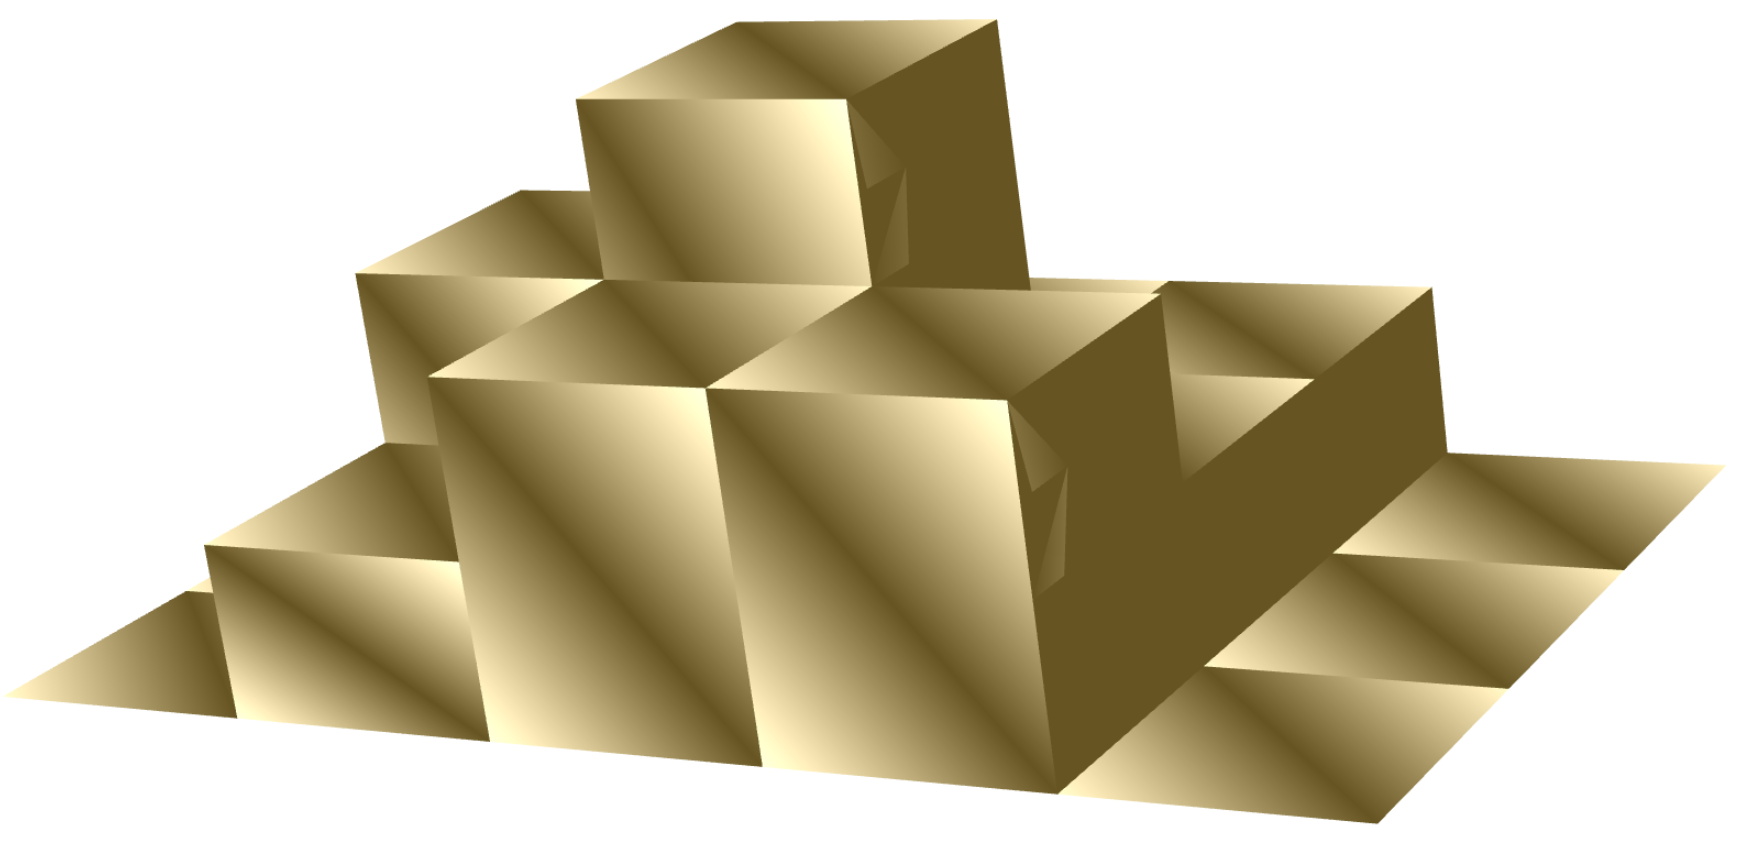
\includegraphics[width=\linewidth]{figures/terrain.png}
    \caption{Example orthogonal terrain.}
    \label{fig:terrain}
    \vspace{-1.2em}
\end{wrapfigure}
In this section, we outline a construction of orthogonal terrains with arbitrary rational extrusion heights.
In our construction, the cross section at will always be on the $x-z$ plane.
To simplify the presentation, we will consider an uniform $X-Y$ grid,
with arbitrary rational extrusion heights corresponding to every grid square (Figure~\ref{fig:terrain}).
\begin{definition}
An $n\times m$ rational grid extrusion is a 3-dimensional structure,
whose projection onto the $x-y$ plane forms an unit grid of size $n\times m$.
In the 3-dimensional structure, the unit face corresponding to the location $(i.j)$,
exists at height $E_{i,j}$ (in the $z$ direction), where $E_{i,j}$ is a rational number.
\end{definition}
%In the case that $E_{i,j}$ is rational, we can simply scale down down our construction by an appropriate size, to obtain integer heights.

\graphicspath{{./figures/}}
\begin{wrapfigure}[7]{r}{0.5\textwidth}
    \vspace{-2.5em}
    \def\svgwidth{0.5\textwidth}
    \input{./figures/column_extrusion.pdf_tex}%
    \caption{Column extrusion with heights $\left\{ 0,1,3,1,2,0\right\}$.}
    \label{fig:column_extrusion}
    \vspace{-0.8em}
\end{wrapfigure}
We consider each ''column'' of a given grid extrusion separately
as an individual \emph{column extrusion} (Figure~\ref{fig:column_extrusion}).
We will construct each of the $n$ columns independently (Figure~\ref{fig:level_shift}),
and attach them together with \emph{column connectors} (Figure~\ref{fig:column_connector}).

We begin by choosing an $2\varepsilon=1/K$ where $K$ is a positive integer.
This is chosen such that $E_{i,j}$ is an integral multiple of $2\varepsilon$ for all $i,j$.
%Given a strip of size $X\times T$, we will consider the evolution of a cross section of length $X$ evolving for time $T$.
%Imagine that there are $T = \frac Y\varepsilon$ time steps of length $\varepsilon$, over which the cross section evolves along the $y$-axis.

\subsection{Construction of Column Extrusion by Level Shifting}
\label{sec:column_extrusion}

First, we consider a single column (Figure~\ref{fig:column_extrusion})
of the orthogonal terrain $\left\{ E_{i,1}, E_{i,2}, \dots, E_{i,n} \right\}$.
We denote the column extrusion heights as $\left\{ H_1, H_2,\dots, H_n \right\}$, where $H_j = E_{i,j}$.
Consider the decomposition of $T$ into the following time intervals:% (parallel to the $x$-axis):
\begin{align}
    \label{eq:column_decomposition}
T = 1 + D_1  +  1 + D_2  +  1 + D_3  +\cdots +  1 + D_{m-1}  +  1.
\end{align}
Here, the time corresponding to the $i$th 1 is realized as the surface at height $H_i$,
and the time corresponding to $D_i = \left| H_i-H_{i+1}\right|$ is the transition between $H_i$ and $H_{i+1}$.

\graphicspath{{./figures/}}
\begin{figure}[htb]
    \def\svgwidth{1.0\textwidth}
    \input{./figures/level_shift_layers.pdf_tex}%
    \caption{
    Cross section change from level $i$ to $i+1$. The \emph{accordion segments} are separated for illustration.
    In reality, the accordion is folded flat. Zero distances are marked by $\phi$.
    The velocities of horizontal and vertical segments are shown by purple and green arrows respectively.
    }
    \label{fig:level_shift_layers}
\end{figure}

\graphicspath{{./figures/level_shift/}}%
\begin{figure}[t!]%
    \centering
    \begingroup%
        \def\svgwidth{0.25\textwidth}
        \captionsetup[subfigure]{width=0.25\textwidth}
        \subfloat[Higher initial level. Top segment moves down.]{%
            \input{./figures/level_shift/column0.pdf_tex}
            \label{fig:level_shift0}
        }%
    \endgroup
    \subfloat[Two segments created. New segments are aligned with top segment, and move down. Vertical segments move inwards.] {%
        \def\svgwidth{0.24\textwidth}
        \input{./figures/level_shift/column1.pdf_tex}%
        \def\svgwidth{0.25\textwidth}
        \input{./figures/level_shift/column2.pdf_tex}%
        \label{fig:level_shift1}
    }%
    \def\svgwidth{0.25\textwidth}
    \subfloat[Two more segments created. Vertical segments reverse direction.] {%
        \input{./figures/level_shift/column3.pdf_tex}%
    %}%
        \def\svgwidth{0.27\textwidth}
    %\subfloat[] {
        \input{./figures/level_shift/column4.pdf_tex}%
    %}%
        \def\svgwidth{0.29\textwidth}
    %\subfloat[] {
        \input{./figures/level_shift/column5.pdf_tex}%
        \label{fig:level_shift2}
    }%

    \subfloat[Level shift completed with four new horizontal segments.] {%
        \def\svgwidth{0.30\textwidth}
        \input{./figures/level_shift/column6.pdf_tex}%
        \def\svgwidth{0.35\textwidth}
        \input{./figures/level_shift/column7.pdf_tex}%
        \label{fig:level_shift3}
    }%
    \begingroup
        \def\svgwidth{0.25\textwidth}
        \captionsetup[subfigure]{width=0.24\textwidth}
        \subfloat[Flat folded state.]{%
            \input{./figures/level_shift/column8.pdf_tex}%
            \label{fig:level_shift4}
        }%
    \endgroup%
    \caption{Level Shifting Gadget. The separation along the $Y$ direction illustrates the layering. The red line denotes the boundary of the cross section.}
    \label{fig:level_shift}
\end{figure}%
%

To construct the column, we will present a cross section sequence. First we describe a \emph{down-shift} gadget.
That is, consider $i$, such that $H_{i+1} = H_i-2\varepsilon\cdot d < H_i$.
Figure~\ref{fig:level_shift_layers} shows the cross section evolution.
This cross section comprises of a two vertical lines separated by a top horizontal line.
The vertical lines are connected to the top segment with
a sequence of $2k$ horizontal segments that \emph{accordion} back and forth.
During each $1$-interval, all segments move along the positive $y$ direction (Figure~\ref{fig:level_shift0}),to create the $i$th level.
Subsequently, during the level shift, all segments move in the $x$-$z$ plane (Figure~\ref{fig:level_shift1},~\ref{fig:level_shift2}).
\begin{restatable}{pro}{AccordionEven}
\label{pro:accordion_even}
The number of accordion folds during horizontal evolution (along the $y$ axis) must be even.
\end{restatable}

The top segment moves downwards in intervals of $2\varepsilon$.
During this process, the horizontal segments move downwards continuously (Figure~\ref{fig:level_shift1},~\ref{fig:level_shift2}).
For the first $\varepsilon$ time interval, a new horizontal downwards moving accordion segment of length zero is created at both accordions,
and the vertical segments move towards each other along the $x$-axis (Figure~\ref{fig:level_shift1}).
For the next $\varepsilon$ time interval, similar (oppositely oriented) accordion segments are created at the lowest position.
This time, the vertical segments move outwards (Figure~\ref{fig:level_shift2}),
until they reach their original position (Figure~\ref{fig:level_shift3}).
Overall, two sets of accordion segments on either side are added, and the height of the top segment decreases by $2\varepsilon$.

In the case that $H_{i+1} = H_i+2\varepsilon\cdot d$, the level up-shift
is simply the down-shift evolution in reverse (Figure~\ref{fig:column_connector}).
This transition is only possible if the initial number of accordion segments in the $H_i$ cross section is at least $2d$.
Specifically, assuming that the minimum height is zero, we have the following lemma.
%This gives us the following lemma.
\begin{lemma}
\label{lem:layer_change}
If the number of accordion segments at level $H_i$ is $l_i$,
then the number of accordion segments after transitioning to level $H_{i+1}$ is $l_{i+1} = l_i - (H_{i+1}-H_i)/\varepsilon$.
Specifically, if the number of layers at level $0$ is $l$, then the number of layers
at level $\max\left\{ H_i\right\}$ is $l - \max\left\{ H_i\right\}/\varepsilon$.
%Specifically, if the number of layers at level $\min\left\{ H_i\right\}$ is $L$, then the number of layers
%at level $\max\left\{ H_i\right\}$ is $L - \left( \max\left\{ H_i\right\}-\min\left\{ H_i\right\} \right)/\varepsilon$.
\end{lemma}
\begin{corollary}
\label{cor:layer_limit}
Since the number of accordion segments can never be negative, the minimum number of layers at at level zero
is $L = \max\left\{ H_i\right\}/\varepsilon$. This also ensures that every other level shift is also possible.
%is $L = \left( \max\left\{ H_i\right\}-\min\left\{ H_i\right\} \right)/\varepsilon$. This also ensures that every other level shift is also possible.
\end{corollary}
\begin{corollary}
\label{cor:column_cross_section_length}
The length of the cross section at a zero level is at least $1 + 2\cdot L\cdot \varepsilon$.
So, the minimum possible length of the cross section under our construction is $1 + 2\cdot\max\left\{ H_i\right\}$.
\end{corollary}

This provides the minimum width of any strip required to construct a column extrusion.
Also the minimum required strip length is given by
$$ T = 1 + D_1  +  1 + D_2  +  1 + D_3  +\cdots +  1 + D_{m-1}  +  1 = m + \sum^{m-1}_{i=1} \left| H_{i+1}-H_i\right|. $$

\begin{restatable}{thm}{column_extrusion}
\label{thm:column_extrusion}
A given column extrusion with heights $\left\{ H_1, H_2,\dots, H_n \right\}$, can be constructed from a strip of paper with size
$X\times T$, where
\begin{align*}
X\ge 1 + 2\cdot\max\left\{ H_i\right\}, && T \ge \left( m + \sum\limits^{m-1}_{i=1} \left| H_{i+1}-H_i\right|\right).
\end{align*}
%X\ge 1 + 2\cdot\left( \max\left\{ H_i\right\}-\min\left\{ H_i\right\}\right) &&T \ge \left( m + \sum\limits^{m-1}_{i=1} \left| H_{i+1}-H_i\right|\right)
\end{restatable}

\subsection{Size of Construction}
\label{sec:size}

We define $M_i = \max_j\left\{ E_{ij}\right\}$.
From Proposition~\ref{prop:accordion_layers}, we know that each column extrusion strip
$\mathcal C^{(i)}$ has width $\left( 1 + 2\cdot\max_j\left\{ E_{ij}\right\}\right) = 1+2\cdot M_i$.
We can ignore the left, and right vertical strips for the leftmost, and rightmost columns.
So, the leftmost and rightmost columns use strips of width $(1 + M_0)$ and $(1 + M_n)$ respectively.

Additionally, we have $n-1$ strip connecors, each of width $2\varepsilon$.
So, the total width of the orthogonal terrain construction is
$$X = 2(n-1)\cdot\varepsilon + n + 2\cdot\sum\limits_{i=1}^n M_i - M_0 - M_n$$
Now, note that our construction is also valid for any $\varepsilon' = \varepsilon/(2k)$, where $k$ is an integer.
In other words, we can make $\varepsilon$ arbitrarily small.

\begin{theorem}
\label{thm:grid_extrusion}
Using the time evolution ($y$ dimension) from Proposition~\ref{prop:accordion_layers},
we conclude that a grid extrusion can be folded from a strip of size $X\times T$, where
\begin{align}
X = n + 2\cdot\sum\limits_{i=1}^n M_i - M_0 - M_n + o(1) && T = m + \sum\limits^{m-1}_{j=1} D_j
\end{align}
\end{theorem}

\subsection{Optimality}
\label{sec:optimality}

Consider a $n\times n$ orthogonal terrain where the highest points along $x$-axis are $M = \max_j E_{ij}$,
and the maximum deltas along the $y$-axis are $D_j = \max_i{\|E_{i,j}-E_{i,j+1}\|} = M$.
Now, we consider a sort of worst case orthogonal terrain defined as follows.
$$
E_{ij}=
\begin{cases}
M, \textrm{ if $(i+j)$ is even}\\
0, \textrm{ if $(i+j)$ is odd}
\end{cases}
$$

This forms a checkerboard alternating between the minimum and maximum heights.
The longest line formed along either axis is the total length of the top surfaces plus the sum of the height changes across the axis, which gives
$$L = n + \sum^{n}_{i=1} M = n + (n-1)\cdot M$$
Assuming that the top faces of the terrain form axis aligned squares in the unfolded state,
we conclude that the minimum required size of the folding is $L\times L$.

From Theorem~\ref{thm:grid_extrusion}, we know that the terrain can be folded from a $X\times Y$ strip of paper,
where $X = n + 2(n-1)\cdot M + o(1)$ and $Y = n + (n-1)\cdot M$.
Since $Y = L$, and $X < 2L$ (assuming an appropriately small value of $\varepsilon$),
or construction results in a folding is within a factor two of the optimal paper usage, under the aforementioned assumption.

%\begin{claim}
%The $x$-axis length of the strip of paper required to fold this shape can be made arbitrarily close to $X$.
%\end{claim}
%\begin{claim}
%The $y$-axis length of the strip of paper required to fold this shape will be exactly $Y$.
%\end{claim}

%First, we pick an $\epsilon$, such that $2\varepsilon$ divides all extrusion heights.
%The construction will require paper of size $X'\times Y$, where $X' = X + 2\epsilon(n-1)$.

%There are two components to the construction
%\begin{itemize}
	%\item $n$ strips parallel to the $y$-axis. Each of these strips will fold to the corresponding strip in the extruded graph. The total area of these strips will be $X\times Y$.
    %\item $n-1$ Intermediate strips, each of size $2\epsilon\times Y$ to connect the main strips together.
%\end{itemize}
%The total area is therefore $X\times Y + (n-1)2\epsilon\times Y = X'\times Y$. This can of course be made arbitrarily close to $X\times Y$.


%\subsection{Removing the Zero Level Assumption}
\label{sec:zero_level_assumption}



%\subsection{Non-Uniform Grids}
\label{sec:non_uniform}



